\documentclass[a0paper,portrait]{baposter}



\usepackage{wrapfig}
\usepackage{lmodern}

\usepackage[utf8]{inputenc}
\usepackage[T1]{fontenc}


\selectcolormodel{RGB}

\graphicspath{{figures/}} % Directory in which figures are stored


\newcommand{\compresslist}{%
\setlength{\itemsep}{0pt}%
\setlength{\parskip}{1pt}%
\setlength{\parsep}{0pt}%
}

\newenvironment{boenumerate}
  {\begin{enumerate}\renewcommand\labelenumi{\textbf\theenumi.}}
  {\end{enumerate}}



\begin{document}


%\definecolor{darkblue}{cmyk}{1,0.31,0,0.32}
%\definecolor{lightblue}{cmyk}{1,0.31,0,0.32}
\definecolor{darkblue}{RGB}{0,120,174}
\definecolor{lightblue}{RGB}{0,120,174}

\begin{poster}
{
grid=false,
headerborder=open, 
colspacing=1em, % Column spacing
bgColorOne=white,
bgColorTwo=white, % Background color for the gradient
borderColor=darkblue, % Border color
headerColorOne=lightblue, % Background color for the header in the content boxes (left side)
headerColorTwo=lightblue, % Background color for the header in the content boxes (right side)
headerFontColor=white, % Text color for the title of box
boxColorOne=white, % Background color of the content boxes
textborder=rounded, % or rectangle, % Format of the border around content boxes, can be: none, bars, coils, triangles, rectangle, rounded, roundedsmall, roundedright or faded
eyecatcher=false, % Set to false for ignoring the left logo in the title and move the title left
headerheight=0.11\textheight, % Height of the header
headershape=rounded, % Specify the rounded corner in the content box headers, can be: rectangle, small-rounded, roundedright, roundedleft or rounded
headershade=plain,
headerfont=\Large\textsf, % Large, bold and sans serif font in the headers of content boxes
%textfont={\setlength{\parindent}{1.5em}}, % Uncomment for paragraph indentation
linewidth=2pt % Width of the border lines around content boxes
}
{}
%
%----------------------------------------------------------------------------------------
%	TITLE AND  NAME
%----------------------------------------------------------------------------------------
%
{
\textsf %Sans Serif
{\color{lightblue}{CFD -- Polymer Stretching by Turbulent \\Flow Field}
}
} 
{\sf\vspace{0.5em}\\
Marco Ghiani$^\dagger$, Paul Grassia and Demosthenes Kivotides
\vspace{0.1em}\\
\small{$\dagger$ Department of Chemical and Process Engineering, University of Strathclyde (Glasgow, UK) 
\vspace{0.2em}\\
marco.ghiani@strath.ac.uk}
}
{\includegraphics[width=3.8cm]{strath.pdf}} % University logo


\headerbox{1. Introduction}{name=introduction,column=0,row=0, span=3}{
\footnotesize{
A polymer is a substance composed of molecules characterized by the multiple repetition of one or more species of atoms or group of atoms (called monomers) linked to each other in amounts sufficient to provide a set of properties that do not vary markedly with the addition of one or a few constitutional repeating units. The polymeric (visco-elastic) fluid have several properties
that makes its studies important in different sectors of industry. 
One of the most interesting properties regards the so called \textit{``Toms effect''}: that is the property to reduce a flow's drag force by introducing a very small amount (one part per milion) of polymers in the fluid.
This properties allows to drastically reduce the energy required to pump a fluid into pipe or channel, with a notable decrease of the costs.

The study of polymer liquids it is very relevant for Chemical Enginnering, since in chemical plant this property is largely used. 
Even though this property is known from the 1940s it is still not well understood, and so the research of polymeric liquids is very interesting for the science and industry. Particular intersest is given to the polymer stretching phenomena, that take place more often in the near wall flow, but experimental studies~\cite{tizia} have demonstrated that this happens also under certain conditions in the turbulent flow homogeneous and isotropic regime.     
In this first part of the research project we are study the stretching phenomena studing a realistic case, studied experimentally, in which the polymers show stretching phenomena under turbulent flow.


}
}


\headerbox{2. Polymer Stretching}{name=model,column=0,below=introduction,span=1}{

%It is important underline that the interaction between the 
\footnotesize{ %Polymer chain in turbulent flow (Hydrodynamic interaction) can be stretched under certain condition: 
%Trouton et al % TODO 
%are the first that gave a comprehensive formulation about this phenomena
Polymer chain in turbulent flow can be stretched under certain condition.
The basic idea of polymer stretching is that this take place when the eigen vector of the strain rate align with the polymer}~\cite{mack,trouton}

{\footnotesize
\[
\underline{\underline\sigma} + \underline{\underline I} P = 2\eta \underline{\underline{\dot{\varepsilon}}} 
\]
}
\footnotesize{Where $\sigma$ is the symmetric stress tensor, $P$ the hydrostatic pressure, $\eta$ the viscosity and $\dot\varepsilon$ the symmetric component of the general strain rate (velocity gradient) tensor $\dot\gamma$. 
The strain rate can be divided into two components,  a symmetric deformation component $\dot\varepsilon_{ij}$ and an antisymmetric rotation component $\omega_{ij}$:
\[
\dot\varepsilon_{ij} = \frac{1}{2} (\dot{\gamma}_{ij}+\dot{\gamma}_{ji})  \quad;\qquad   \omega_{ij} = \frac{1}{2} (\dot{\gamma}_{ij}-\dot{\gamma}_{ji})
\label{eq:epsil}
\]
}
\vspace{-0.24in}
\begin{center}
    \includegraphics[width=.9\linewidth]{shear.png}
\end{center}
\vspace{-0.18in}
\footnotesize{The rotation (spin motion) does not contribute to the chain stretching indeed the strain rate (high strain rate at lower turbulent scale) 
\[
\varepsilon_{ij} \vec{\lambda} = \lambda_i \vec{\lambda_i} \qquad  i=1,2,3
\]
}
\footnotesize{Where $\vec{\lambda}$ and $\lambda$ are the eigenvector and eigen value respectly. $\lambda_1 > 0 $ always, considering a polymer of length $= l$ we can say that the stretching phenomena happens when: % the order of interpolation that are computed during the iteration.
\[
\vec{\lambda_1} \cdot \vec{l} \neq 0  \qquad \frac{\vec{\lambda_1} \cdot \vec{l}}{|\lambda||l|} = \cos\theta \neq 0 
\]
}
\footnotesize{
It is very important to know the eigenvectors and the $\cos\theta$. When we have
$\cos\theta \pm 1 $, the polymer stretching is maximum.
}

}


\headerbox{6. Polymer Result}{name=mcs,column=0,below=model,span=1}{
\footnotesize{
%To measure similarity of two molecules or to combine them into one model, DeCAF first finds their \textbf{maximum common substructure (MCS)}.
%To provide fast, but accurate method for solving MCS problem, we combined Generic Match Algorithm (GMA) \cite{xu1996gma} with backtracking algorithm proposed by Yiqun Cao \cite{cao2008maximum}.

%Here we present comparison of molecules with similar and with different structures.
%DeCAF scores and \textbf{Tanimoto coefficient (Tc)} values are shown in red and black, respectively.
\hspace{-0.1in}
\includegraphics[width=1.05\linewidth]{stretching.pdf}
\footnotesize{
The above picture shown polymer in three different configuration from equilibrium configuration to stretch configuration, This behavior is due to the interaction with the turbulent smaller eddies. } 

}
%\begin{center}
%    \includegraphics[width=\linewidth]{sim}
%\end{center}
}

\headerbox{3. Mathematical Model}{name=screen,span=2,column=1,below=introduction}{ % To reduce this block to 1 column width, remove 'span=2'
\footnotesize{
Hydrodynamic interactions (Polymer-Water) take place at smaller scales then the turbulence eddies cascade~\cite{demos}. In order to study this scale we have to fully resolve the turbulence spectrum (DNS)
using an in-House Fortran90 code. We solved a coupling system of Navier-Stokes \textit{(fluid)} and Langevin equation \textit{(Polymer)}~\cite{demos2}. 
}
\footnotesize{
\begin{equation}
 \frac{\partial \bar{u}_i}{\partial t} = 0  ;\qquad
   \rho  \frac{\partial \bar{u}_i}{\partial t} + \rho \frac{\partial (\bar{u}_i \bar{u}_j) }{\partial x_j}+\frac{\partial\bar{p}}{\partial x_i} + \rho \frac{\partial (\overline{u'_i u'_j})}{\partial x_j} 
= \mu \frac{\partial^2 \bar{u}_i}{\partial^2 x_j } + ^d\!F_i^k \, G_{\xi} (\mathbf{x}-\mathbf{r}^k) = 0\\
  \label{eq:2}
\end{equation}

\begin{equation}
  ^i\!F_i^k \, + ^e\!F_i^k \, + ^m\!F_i^k \, + ^d\!F_i^k \,+ ^t\!F_i^k = 0
\label{eq:langevin}
\end{equation}

\begin{equation}
    \frac{\partial u_i^\mathcal{S}}{\partial x_i} = 0 ; \qquad \frac{\partial p^{\mathcal{S}}}{\partial x_i} - \mu \frac{\partial^2 u_i^{\mathcal{S}}}{\partial^2 x_j} - \, ^d\!F_i^k \delta(\mathbf{x} -\mathbf{r}^k) = 0
    \label{eq:st}
\end{equation}
\begin{equation}
\overline{u'_i u'_j}(\mathbf{x}) = \overline{(u_l^{\mathcal{S}})_i 
(u_l^{\mathcal{S}})_j }(\mathbf{x}) = \int_V (u_l^{\mathcal{S}})_i
(\mathbf{x-x'}) (u_l^{\mathcal{S}})_j (\mathbf{x-x'})G_\xi (\mathbf{x'})d\mathbf{x'}
\label{eq:6}
\end{equation}
\vspace{-0.08in}

Where Eq~\ref{eq:2} is the Navier Stokes equtions, Eq.~\ref{eq:langevin} is the stochastic Langevin equation, Eq.~\ref{eq:st} are the creeping flow (Stokes equations), and Eq.~\ref{eq:6}  describe the residual stress in~\ref{eq:2} in terms of local a local field $u_l^\mathcal{S}$



We deal with Homogeneous and Isotropic Turbulence, that is the flow condition present in the center of a channel in the turbulent ``wake'' regime ($y^+$ curve).
}


%\vspace{-5pt}
%\begin{center}
%    \includegraphics[width=0.85\linewidth]{screen}
%\end{center}
}


\headerbox{4. Method of Solution}{name=sea,span=2,column=1,below=screen}{ % To reduce this block to 1 column width, remove 'span=2'

%\begin{wrapfigure}{l}{0.3\textwidth}
%    \vspace{10pt}
%    \begin{center}
%        \includegraphics[width=\linewidth]{class}
%    \end{center}
%    %\vspace{-145pt}
%\end{wrapfigure}

\footnotesize{
We solve the system of equations using a in-House Fortran code, that uses a FVM (Finite Volume
Method) approach for discretizing the system in a staggered cubic grid with 256$^3$ computational cell,
the accuracy of the solver is first order for the time-marching and second order semi-Implicit method
for space. Brownian Stochastic Dynamics is used for the Polymer, that interacts with the flow by
computing the Langevin Equation. The Flow is Homogeneous Isotropic Turbulent, and we forced the
flow to be in a steady state compute a previous purely Fluid dynamic simulation in order to reach 
suitable Reynolds number (based on a Taylor microscale) and then using this condition of flow to
initialize the fluid-polymer computations, in this way, we obtain a steady state homogeneous isotropic
turbulence which allows us to study the hydrodynamic interaction between polymer and solvent.% We use a polyethylene oxide (PEO) water solution that is experimentally well investigated~\cite{tizia} and show
%that the polymer stretch in homogeneous isotropic turbulence at the highest turbulence spectrums of
%frequency
}


% Please ask me about details.

%\hspace{0pt}\includegraphics[width=0.95\linewidth]{res}

}
\headerbox{5. Result}{name=result,column=1,below=sea,span=2}{
\begin{wrapfigure}{l}{0.2\textwidth}
    \vspace{-16pt}
    \begin{center}
        \includegraphics[width=\linewidth]{contours2}
    \end{center}
   \vspace{150pt}
\end{wrapfigure}

\footnotesize{
%We use a polyethylene oxide (PEO) water solution that is experimentally well investigated~\cite{tizia} and show that the polymer stretch in homogeneous isotropic turbulence at the highest turbulence spectrums of frequency.

Results for the Turbulent iso-surface of Vorticity 30\% of the maximum value (A), and Vorticity 70\% of the maximum value (B) have been reported in figure. It is possible to observe that also using a $Re_\lambda$ relatively small ($\approx$ 100) the vorticity is increased, this is due to the fact that we are resolving all the turbulent spectrum starting from the smaller scale, called the ``Kolmogorov scale $\eta$'' (upper turbulence spectrum of frequency) to the largest called ``Large Eddy Turn over''.
The plot below reports the steady state turbulent flow with which we initialize the Polymer-Fluid simulations (left). It is possible to observe that the flow reaches the steady state after a certain period of time, this period of time is almost equal to thirty times the Large eddy turnover. The plot on the right is the turbulence spectrum, highlighting the viscous cut-off regime it is the area in which we would that the polymer chain reside in order to be stretched as also reported in the study of Vonlanthen et al~\cite{tizia} 


%\begin{wrapfigure}{l}{0.5\textwidth}
    \hspace{-18pt}
    %\begin{center}
        \includegraphics[width=0.6\linewidth]{turbulence}
        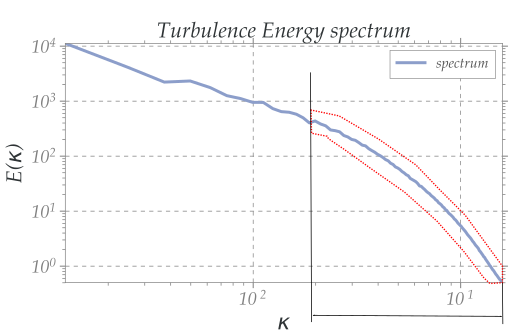
\includegraphics[width=0.45\linewidth]{spectra2}
    
    %\end{center}
    \vspace{14pt}
%\end{wrapfigure}

}




% DeCAF is a chemoinformatical tool that can be helpful in ligand-based drug design.
% It provides a comprehensive molecule description and a fast algorithms for comparing and aligning multiple ligands.
% It can be also used in other [procedures], such as database screening or drug repositioning.
% DeCAF is written in Python and freely available at \textbf{\color{darkblue}http://bitbucket.org/marta-sd/decaf}. 


}



\headerbox{7. Conclusions}{name=conclusion,column=1,below=result,span=2,above=bottom}{
\scriptsize{
The aims of this project is to better understand the Polymer dynamics in a Turbulent homogeneous and isotropic flow. 
We now have concluded that:
\begin{itemize}
    \item We had calculated all the quantities that represent the experiments condition ~\cite{tizia}
    \item We have computed a Turbulence statistically steady state Flow 
    \item We now are moving on perform a simulations including polymers. 
    \item We have the software facility to show the behaviour of polymer under the influence of the surrounding flow (Demonstrate using movie of the polymer evolution).
\end{itemize}
}
}

\headerbox{8. References}{name=references,column=0,span=1,below=mcs,above=bottom}{


%\small % Reduce the font size in this block
\renewcommand{\section}[2]{\vskip 0.05em} % Get rid of the default "References" section title
%\nocite{*} % Insert publications even if they are not cited in the poster

\scriptsize{
\bibliographystyle{unsrt}
\bibliography{poster} % Use sample.bib as the bibliography file
}
}

\end{poster}

\end{document}
